\documentclass[10pt]{article}
\usepackage[margin=1in]{geometry}
\usepackage[T1]{fontenc}
\usepackage{lmodern}
\usepackage{amsmath,amssymb,amsthm}
\usepackage{graphicx}
\usepackage{booktabs}
\usepackage{xcolor}
\usepackage[colorlinks=true,linkcolor=blue!50!black,citecolor=blue!50!black,urlcolor=blue!50!black]{hyperref}
\usepackage[numbers,sort&compress]{natbib}
\usepackage{microtype}
\usepackage{enumitem}
\setlist{itemsep=1pt,topsep=2pt}

\newtheorem{theorem}{Theorem}
\newtheorem{proposition}[theorem]{Proposition}
\newtheorem{lemma}[theorem]{Lemma}
\newtheorem{corollary}[theorem]{Corollary}
\newcounter{algo}
\renewcommand{\thealgo}{\arabic{algo}}
\theoremstyle{remark}
\newtheorem{remark}{Remark}

% generated by make_numbers.py -- do not edit
\newcommand{\AccDiffP}{0.40}
\newcommand{\AccDiffScanSerial}{-0.2\pm0.6}
\newcommand{\AccLongSJ}{78.6}
\newcommand{\AccLongScan}{77.7}
\newcommand{\AccLongSerial}{77.9}
\newcommand{\AccSJ}{73.5\pm0.6}
\newcommand{\AccScan}{73.3\pm0.7}
\newcommand{\AccSerial}{73.5\pm0.5}
\newcommand{\AlifMonoChecks}{14{,}048}
\newcommand{\AlifMonoViol}{0}
\newcommand{\AllenCells}{14}
\newcommand{\AllenDiff}{+0.024}
\newcommand{\AllenFHard}{0.442}
\newcommand{\AllenFNo}{0.047}
\newcommand{\AllenFSoft}{0.417}
\newcommand{\AllenFracRel}{63}
\newcommand{\AllenHardWins}{10}
\newcommand{\AllenP}{0.22}
\newcommand{\AllenRel}{0.701}
\newcommand{\AllenSpeed}{11.0}
\newcommand{\AllenT}{140{,}032}
\newcommand{\AutoCells}{14}
\newcommand{\AutoGradRel}{0}
\newcommand{\AutoMax}{27}
\newcommand{\AutoMin}{1.00}
\newcommand{\AutoScanMin}{0.63}
\newcommand{\AutoSpikesEq}{all}
\newcommand{\BigAllDiff}{-0.015}
\newcommand{\BigAllHard}{0.302}
\newcommand{\BigAllN}{78}
\newcommand{\BigAllNo}{0.033}
\newcommand{\BigAllP}{0.0027}
\newcommand{\BigAllRel}{0.450}
\newcommand{\BigAllSoft}{0.318}
\newcommand{\BigAllWins}{18}
\newcommand{\BigAspinyDiff}{-0.009}
\newcommand{\BigAspinyHard}{0.369}
\newcommand{\BigAspinyN}{47}
\newcommand{\BigAspinyNo}{0.041}
\newcommand{\BigAspinyP}{0.18}
\newcommand{\BigAspinyRel}{0.560}
\newcommand{\BigAspinySoft}{0.378}
\newcommand{\BigAspinyWins}{15}
\newcommand{\BigChunks}{2}
\newcommand{\BigNFbNine}{0.54--0.57}
\newcommand{\BigNFbNineNine}{0.52--0.56}
\newcommand{\BigSpinyDiff}{-0.026}
\newcommand{\BigSpinyHard}{0.201}
\newcommand{\BigSpinyN}{31}
\newcommand{\BigSpinyNo}{0.023}
\newcommand{\BigSpinyP}{0.0012}
\newcommand{\BigSpinyRel}{0.284}
\newcommand{\BigSpinySoft}{0.227}
\newcommand{\BigSpinyWins}{3}
\newcommand{\FbMaxNine}{31}
\newcommand{\FbMaxNineNine}{30}
\newcommand{\FbMaxSpeedup}{31}
\newcommand{\FireRateLong}{0.02}
\newcommand{\FireRateShort}{0.38}
\newcommand{\FitHardErrMax}{4.4\times10^{-4}}
\newcommand{\FitMsAutoMillion}{51}
\newcommand{\FitMsAutoShort}{2.1}
\newcommand{\FitMsSerialMillion}{449}
\newcommand{\FitMsSerialShort}{24.5}
\newcommand{\FitSameAll}{identical}
\newcommand{\FitSpeedMax}{11.9}
\newcommand{\FitSpeedMin}{8.9}
\newcommand{\FwdMaxNine}{7.8}
\newcommand{\FwdMaxNineN}{128}
\newcommand{\FwdMaxNineNine}{7.6}
\newcommand{\FwdMaxNineNineN}{128}
\newcommand{\FwdMaxNineNineT}{65{,}536}
\newcommand{\FwdMaxNineT}{65{,}536}
\newcommand{\FwdMaxSpeedup}{7.8}
\newcommand{\FwdWinMaxNNine}{1{,}024}
\newcommand{\FwdWinMaxNNineNine}{1{,}024}
\newcommand{\GradRelSJLong}{9.5\times10^{-5}}
\newcommand{\GradRelSJShort}{7.5\times10^{-7}}
\newcommand{\GradRelScanLong}{5.8\times10^{-7}}
\newcommand{\GradRelScanShort}{1.2\times10^{-7}}
\newcommand{\LongCellsNine}{7}
\newcommand{\LongCellsNineNine}{7}
\newcommand{\LongFbMaxNine}{37}
\newcommand{\LongFbMaxNineNine}{35}
\newcommand{\LongFwdMaxNine}{12}
\newcommand{\LongFwdMaxNineNine}{11}
\newcommand{\LongMaxFlipNine}{0}
\newcommand{\LongMaxFlipNineNine}{0}
\newcommand{\LongVFourBestNine}{0}
\newcommand{\LongVFourBestNineNine}{0}
\newcommand{\MaxFlipNine}{0}
\newcommand{\MaxFlipNineNine}{0}
\newcommand{\MaxOvfNine}{0.000}
\newcommand{\MaxOvfNineNine}{0.029}
\newcommand{\MaxPiecesNine}{4.1}
\newcommand{\MaxPiecesNineNine}{5.3}
\newcommand{\NSeedsSJ}{8}
\newcommand{\NSeedsScan}{8}
\newcommand{\NSeedsSerial}{8}
\newcommand{\NoRepairMismatch}{0}
\newcommand{\RepairRoundsLong}{23--35}
\newcommand{\RepairRoundsShort}{4--6}
\newcommand{\SJMaxNine}{111}
\newcommand{\SJMaxNineNine}{111}
\newcommand{\SJMaxSpeedup}{111}
\newcommand{\SJvsSerialSmall}{2.6--3.8}
\newcommand{\ShdAutoMax}{3.0}
\newcommand{\ShdAutoMin}{1.00}
\newcommand{\SoftAllenCells}{9}
\newcommand{\SoftAllenDiverged}{3}
\newcommand{\SoftAllenFOneDiff}{0.000}
\newcommand{\SoftAllenMsScan}{2}
\newcommand{\SoftAllenMsSerial}{26}
\newcommand{\SoftAllenParamDiff}{5.1\times10^{-5}}
\newcommand{\SoftAllenSpeed}{10.4}
\newcommand{\SoftAllenSpeedMax}{10.9}
\newcommand{\SoftAllenSpeedMin}{9.9}
\newcommand{\SoftAllenTested}{12}
\newcommand{\SoftMax}{4.1}
\newcommand{\SoftMaxBeta}{0.95}
\newcommand{\SoftMaxFlip}{3.0\times10^{-7}}
\newcommand{\SoftMaxN}{4}
\newcommand{\SoftMaxT}{262{,}144}
\newcommand{\SpikeMisSJLong}{3.0\times10^{-6}}
\newcommand{\SpikeMisSJShort}{0}
\newcommand{\SpikesEqScanLong}{all}
\newcommand{\SpikesEqScanShort}{all}
\newcommand{\SscAccSJ}{65.0\pm0.4}
\newcommand{\SscAccScan}{64.9\pm0.2}
\newcommand{\SscAccSerial}{64.9\pm0.3}
\newcommand{\SscDiff}{+0.0}
\newcommand{\SscGradRelSJ}{1.9\times10^{-4}}
\newcommand{\SscGradRelScan}{3.8\times10^{-8}}
\newcommand{\SscNSJ}{3}
\newcommand{\SscNScan}{3}
\newcommand{\SscNSerial}{3}
\newcommand{\SscSpikesEqScan}{all}


\title{Hard Resets Compose: Exact Time-Parallel Spiking Neurons\\ via Piecewise-Affine Map Scans}
\author{Anonymous Authors}
\date{}

\begin{document}
\maketitle

\begin{abstract}
The hard reset of a leaky integrate-and-fire (LIF) neuron is widely seen as what prevents spiking networks from being parallelized over time: it makes the state update non-linear and apparently non-associative.
Existing time-parallel methods therefore remove the reset, soften it, relax the spike function and iterate, or commit one output spike per chunk.
We show that this is unnecessary in discrete time.
As a function of the incoming membrane potential, the state map of a hard-reset LIF neuron over $L$ steps is affine below a threshold and piecewise constant above it, with at most $L+1$ pieces, and this family is closed under composition, so the recurrence is an associative scan over piecewise-affine maps.
We give a closed form for these maps, show that the bound is tight, and prove that the corresponding tight bound for soft reset is quadratic, $1+L(L+1)/2$: in map space the hard reset is the easier nonlinearity.
Restricted to reachable states, whose lower bound is itself a three-parameter scan, the expected number of pieces is bounded independently of $L$ for leaky neurons; measured maps have 2--5 pieces.
The resulting forward pass is exact, non-iterative, and has a depth independent of the number of spikes; an optional repair step makes it bit-identical to the serial floating-point loop.
On an RTX~5090, against fused serial Triton kernels tuned per configuration, the exact forward is up to $\LongFwdMaxNine\times$ faster and forward+backward up to $\LongFbMaxNine\times$ faster when few neurons run for many steps, and slower once the serial kernel saturates the GPU; we map this crossover.
On SHD and SSC, training with the scan reproduces serial training: spikes are bit-identical, gradients agree to within $10^{-6}$, and accuracy matches within seed noise.
\end{abstract}

% ---------------------------------------------------------------------------
\section{Introduction}

Spiking neural networks (SNNs) are recurrent in time even when they are feed-forward in space: every neuron carries a membrane potential that integrates its input, fires when a threshold is crossed, and is then reset.
Training by back-propagation through time (BPTT) with surrogate gradients~\citep{neftci2019surrogate} therefore unrolls $T$ sequential steps, which makes long sequences slow on parallel hardware.
Linear recurrences --- linear RNNs and state-space models --- avoid this with parallel associative scans~\citep{blelloch1990prefix,martin2018parallelizing,smith2023s5}, and the sub-threshold dynamics of an LIF neuron are linear.
The reset is not.

A sequence of works has looked for ways around the reset.
Parallel spiking neurons~\citep{fang2023psn} remove it; the parallel spiking unit~\citep{li2024psu} and spiking SSMs~\citep{zhong2024spikessm} use soft or estimated resets; fixed-point parallel training~\citep{feng2025fpt} and FidLIF~\citep{he2026fidlif} solve for the trajectory iteratively after relaxing the Heaviside into a sigmoid; Bullet Trains~\citep{morrill2026bullet} keeps the exact hard reset in continuous time by scanning the linear inter-spike dynamics over chunks of input events and committing one output spike per chunk; and a recent system description~\citep{tachyon2026} parallelizes the backward adjoint but states that ``hard resets destroy forward associativity'' and resorts to speculative draft-and-verify forward passes.
All of these approaches treat the reset as a non-associative event to be removed, approximated or worked around.

\paragraph{This paper.}
We observe that the reset is non-associative only in \emph{state space}.
In \emph{map space} --- composing the one-step maps $f_t:u_{t-1}\mapsto u_t$ instead of applying them --- associativity is automatic, and the only question is whether composed maps admit a compact representation.
For the hard reset the answer is yes, and the structure is simple: a segment map is affine for incoming potentials that do not cause a spike in the segment and constant on each interval of potentials that first spike at the same step, because the reset erases all memory of the incoming potential (Fig.~\ref{fig:segmap}).
Our contributions:
\begin{enumerate}[leftmargin=*]
\item \textbf{Structure (Sec.~\ref{sec:structure}).} A closed form for the $L$-step hard-reset segment map: its breakpoints are the strict running minima of $a_k=(\theta-b_k)/\beta^k$, where $b_k$ is the zero-start free trajectory; hence at most $L+1$ pieces, a bound that is attained. The family is closed under composition, and two maps compose by concatenating breakpoint lists and evaluating the right map at the left map's constants. The result holds verbatim for time-varying leaks, thresholds and reset values.
\item \textbf{Hard vs.\ soft (Sec.~\ref{sec:soft}).} For subtractive reset we prove a tight quadratic bound, $1+L(L+1)/2$. The upper bound follows from a lexicographic monotonicity lemma for (spike count, membrane potential); the matching construction uses a constant input and a leak close to 1. Empirically, soft-reset segment maps have up to $30\times$ more pieces than hard-reset ones. In map space, the hard reset is the easier nonlinearity.
\item \textbf{Typical size (Sec.~\ref{sec:domain}).} Only breakpoints inside the reachable state interval matter. A tight lower end of that interval is itself given by a scan over a three-parameter monoid, and under a bounded-density assumption the expected in-domain size is independent of $L$. Measured chunk maps have 2--5 pieces on average for $\beta$ from 0.9 to 1, whatever the chunk length.
\item \textbf{Algorithm and exactness (Sec.~\ref{sec:algo}).} A two-level GPU scan (fold chunks into capacity-$K$ maps, carry scalars across chunks, replay chunks in parallel) whose depth is independent of the spike count, with an exact serial fallback on capacity overflow, and a repair iteration that makes the floating-point output bit-identical to the serial kernel. Combined with the (known) affine-scan backward pass, training is BPTT-equivalent.
\item \textbf{Measurements (Sec.~\ref{sec:exp}).} Exhaustive exact-arithmetic tests, floating-point stress tests, a best-vs-best GPU benchmark against tuned fused serial kernels and SpikingJelly up to $T=262{,}144$, and training on SHD and SSC.
\end{enumerate}
We are explicit about the limits: time-parallelism helps only when the serial kernel cannot fill the GPU (small batch$\times$width, long $T$), the method requires the input currents of a layer to be known in advance (feed-forward connectivity within the layer), and the per-step work of the forward scan grows with the map capacity $K$.

\begin{figure}[t]
\centering
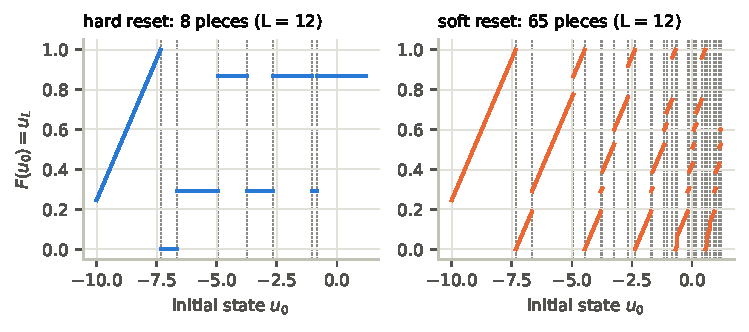
\includegraphics[width=0.92\linewidth]{figs/segment_map.pdf}
\caption{Exact segment maps $u_0\mapsto u_L$ for one random input segment ($L=12$, $\beta=0.9$, $\theta=1$). Left: hard reset --- affine below the leftmost breakpoint, piecewise constant above it (8 pieces; the bound is 13). Right: soft reset on the same input --- every piece is affine and the count is 65 (the bound is 79). Dotted lines: breakpoints.}
\label{fig:segmap}
\end{figure}

% ---------------------------------------------------------------------------
\section{Related work}
\label{sec:related}

\paragraph{Time-parallel SNN training.}
PSN~\citep{fang2023psn} drops the reset and computes the membrane potential as a learnable linear filter; follow-ups add estimated or decoupled resets~\citep{li2024psu,zhong2024spikessm,huang2026paralleltraining}. FPT~\citep{feng2025fpt} iterates a fixed-point map for $K\approx 3$ rounds on a sigmoid-relaxed spike function. FidLIF~\citep{he2026fidlif} applies Newton iterations to the relaxed trajectory equation, each iteration being an associative scan, and reports errors relative to the matched \emph{relaxed} serial dynamics. Bullet Trains~\citep{morrill2026bullet} targets continuous-time event-based LIF neurons; it scans the affine inter-spike dynamics within a chunk of input events, locates the first output spike analytically and with Newton--Raphson, commits it, and restarts the next chunk after it --- so the number of sequential chunk iterations grows with the number of output spikes. Tachyon~\citep{tachyon2026} parallelizes the surrogate-gradient adjoint as an affine scan (as do FidLIF and our backward pass) and uses speculative draft-verify-commit for exact forwards. Our forward pass differs from all of these: it is discrete-time, non-iterative, involves no relaxation, and its depth does not depend on the number of spikes (Table~\ref{tab:methods}).

\begin{table}[t]
\centering\footnotesize
\setlength{\tabcolsep}{4pt}
\begin{tabular}{lcccc}
\toprule
Method & reset & exact & iterative & spike-dependent depth\\
\midrule
PSN~\citep{fang2023psn} & removed & -- & no & no\\
PSU, SPikE-SSM~\citep{li2024psu,zhong2024spikessm} & soft / estimated & no & no & no\\
FPT~\citep{feng2025fpt} & hard, relaxed & no & yes & no\\
FidLIF~\citep{he2026fidlif} & hard, relaxed in solve & no & yes (Newton) & no\\
Bullet Trains~\citep{morrill2026bullet} & hard, continuous time & yes & chunk restarts & yes\\
Tachyon~\citep{tachyon2026} & hard & yes & speculative rounds & yes\\
\textbf{This work} & hard, discrete time & yes & no & no\\
\bottomrule
\end{tabular}
\caption{Time-parallel forward passes for LIF neurons, as described by their authors. ``Exact'': the forward pass agrees with the serial hard-reset recurrence in exact arithmetic. ``Spike-dependent depth'': the number of sequential rounds grows with the number of output spikes.}
\label{tab:methods}
\end{table}

\paragraph{Scans over function compositions.}
Parallel prefix computation applies to any associative operator~\citep{blelloch1990prefix}, including composition of functions from a family with a closed, bounded representation, e.g.\ affine maps (linear recurrences~\citep{kogge1973parallel,martin2018parallelizing}) or finite-state transition functions. Generic nonlinear RNNs lack such a representation, which motivates Newton-type parallelization (DEER/ELK~\citep{lim2024deer,gonzalez2024elk}). Our contribution is to identify that the hard-reset LIF family has such a representation, to bound its size, and to make it practical.

% ---------------------------------------------------------------------------
\section{Setup}

We use the discrete LIF neuron with charge--fire--reset ordering:
\begin{equation}
v_t=\beta u_{t-1}+I_t,\qquad s_t=\mathbb 1[v_t\ge\theta],\qquad u_t=\begin{cases}u_r & s_t=1\ \text{(hard reset)}\\ v_t& s_t=0,\end{cases}
\label{eq:lif}
\end{equation}
with leak $\beta>0$ (typically $\beta\in(0,1]$), threshold $\theta$, reset value $u_r$ and real inputs $I_t$ (of either sign). In a layer, $I_t=Wx_t+b$ is computed for all $t$ at once from the previous layer's spikes, and \eqref{eq:lif} runs independently per neuron and batch element; we denote the number of independent recurrences by $N$ (batch$\times$width). As a function of $u=u_{t-1}$, one step is
\[
f_t(u)=\begin{cases}\beta u+I_t,&u<c_t:=(\theta-I_t)/\beta,\\ u_r,&u\ge c_t.\end{cases}
\]
For a segment $1..L$ write the free (no-spike) trajectory as $\beta^k u_0+b_k$ with $b_k=\sum_{j\le k}\beta^{k-j}I_j$, and define
\[
a_k=\frac{\theta-b_k}{\beta^k},\qquad\text{so that}\qquad u_0\ge a_k\iff \beta^ku_0+b_k\ge\theta .
\]
Let $G_k$ denote the state at the end of the segment when the neuron is reset at step $k$ (obtained by running \eqref{eq:lif} from $u_r$ on $I_{k+1..L}$; $G_L=u_r$). The segment map is $F=f_L\circ\cdots\circ f_1$.

% ---------------------------------------------------------------------------
\section{The structure of hard-reset segment maps}
\label{sec:structure}

\begin{theorem}[closed form]
\label{thm:structure}
Let $m_k=\min_{j\le k}a_j$ ($m_0=+\infty$) and call $k$ a \emph{record} if $a_k<m_{k-1}$. Then $F(u_0)=\beta^Lu_0+b_L$ for $u_0<m_L$, and for consecutive records $k'<k$, $F\equiv G_k$ on $[a_k,a_{k'})$ (and on $[a_{k_1},\infty)$ for the first record $k_1$). In particular $F$ has $1+\#\{\text{records}\}\le L+1$ pieces.
\end{theorem}
\begin{proof}
Let $k^*(u_0)$ be the first spike time in the segment ($\infty$ if none). Before $k^*$ the trajectory is free, so $k^*(u_0)\le k\iff\exists j\le k: u_0\ge a_j\iff u_0\ge m_k$. Hence $\{k^*=k\}=[m_k,m_{k-1})$, which is non-empty exactly when $k$ is a record. On it, $u_k=u_r$ regardless of $u_0$, so $F\equiv G_k$; on $\{k^*=\infty\}=(-\infty,m_L)$, $F$ is the free map.
\end{proof}

Two facts follow directly: the first spike time is non-increasing in $u_0$ (the level sets above are ordered), and the proof uses only $\beta>0$, so it covers negative inputs, any $u_r$, $\beta=1$ (IF neurons) and even $\beta>1$. A one-line consequence of the definition is
\begin{equation}
a_{k+1}-a_k=\frac{(1-\beta)\theta-I_{k+1}}{\beta^{k+1}},
\label{eq:arec}
\end{equation}
so $a$ decreases exactly at steps with suprathreshold drive $I_{k+1}>(1-\beta)\theta$.

\begin{proposition}[tightness]
\label{prop:tight}
For $0<\beta<1$, $\theta>0$, $u_r=0$ and constant input $I\in\big((1-\beta)\theta,\,(1-\beta)\theta/(1-\beta^L)\big)$, $F$ has exactly $L+1$ pieces.
\end{proposition}
\begin{proof}
By \eqref{eq:arec}, $a_k$ is strictly decreasing, so every $k$ is a record. From $u_r=0$ the neuron reaches $I(1-\beta^m)/(1-\beta)<\theta$ after $m\le L$ steps, so it does not fire again after a reset and $G_k=I(1-\beta^{L-k})/(1-\beta)$ are pairwise distinct; no two pieces merge.
\end{proof}

\begin{corollary}[time-varying parameters]
\label{cor:tv}
Let step $t$ be $f_t(u)=\alpha_tu+I_t$ if $\alpha_tu+I_t<\theta_t$ and $f_t(u)=r_t$ otherwise, with $\alpha_t>0$ and arbitrary real $I_t,\theta_t,r_t$. Then Theorem~\ref{thm:structure} holds with $\beta^k$ replaced by $A_k=\prod_{j\le k}\alpha_j$, $b_k$ by the corresponding free response, and $a_k=(\theta_k-b_k)/A_k$.
\end{corollary}
The proof of Theorem~\ref{thm:structure} only uses that the free trajectory is increasing in $u_0$ and that a spike erases $u_0$, so it carries over unchanged. This covers input-dependent leaks (e.g.\ conductance-based input $u\mapsto(\beta-g_t)u+g_tE$ while $\beta-g_t>0$), learned per-step time constants, and thresholds that vary in time but do not depend on the neuron's own spikes. The composition operator is unchanged, since it only manipulates $(A,B)$ pairs. In exact arithmetic, composed maps for random time-varying parameters ($\alpha_t$ also above 1) matched the serial recurrence in all 2000 test cases. Refractory periods also preserve forgetting. After a spike the trajectory no longer depends on $u_0$, so segment maps keep the same form; they must be indexed by the refractory counter at the segment start (we have not implemented this).

\paragraph{Closure and composition.}
Let $\mathcal H$ be the set of maps that are affine with positive slope on $(-\infty,x_0)$ and piecewise constant with finitely many left-closed pieces on $[x_0,\infty)$ (possibly $x_0=+\infty$). The composition of the segment maps of two adjacent segments is the segment map of their concatenation, so by Theorem~\ref{thm:structure}:

\begin{corollary}[monoid]
Segment maps form a monoid under composition, and the composition of maps covering $L_1$ and $L_2$ steps has at most $L_1+L_2+1$ pieces.
\end{corollary}

Concretely, for $F=(A,B;\,x_0<\dots<x_{n-1};\,c_0,\dots,c_{n-1})$ followed by $g=(A',B';\,y_0<\dots;\,d_\cdot)$, the composite $g\circ F$ is
\begin{itemize}
\item affine, $A'A u+A'B+B'$, for $u<\min\big(x_0,(y_0-B)/A\big)$;
\item equal to $d_j$ on the pull-backs $[(y_j-B)/A,(y_{j+1}-B)/A)$ of $g$'s pieces, restricted to $u<x_0$;
\item equal to $g(c_i)$ on $[x_i,x_{i+1})$.
\end{itemize}
Because every pulled-back breakpoint lies below $x_0\le x_i$, the two breakpoint lists are \emph{concatenated, not merged}. The cost is dominated by the $n_F$ point queries $g(c_i)$, so composition takes $O(n_g+n_F\log n_g)$ work and $O(\log n_g)$ depth. Whether a linear-time composition exists is open: the constants $c_i$ are not ordered.

\begin{figure}[t]
\centering
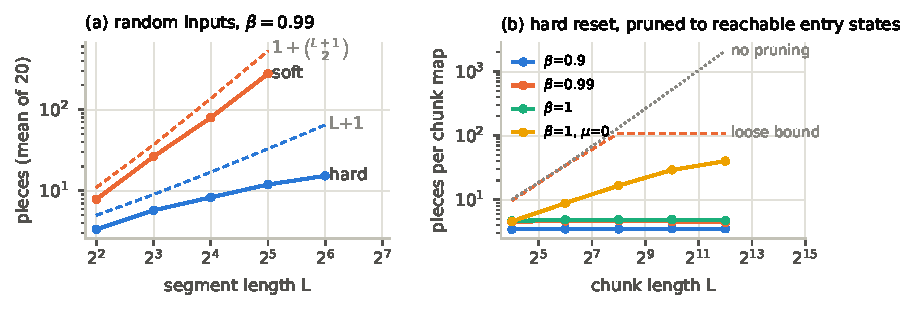
\includegraphics[width=0.95\linewidth]{figs/pieces.pdf}
\caption{(a) Mean number of pieces of exact segment maps for random inputs ($I_t\sim\mathcal N(0.15,0.3^2)$, 20 draws per point, exact rational arithmetic). Dashed lines: the worst-case bounds $L+1$ (hard) and $1+L(L+1)/2$ (soft); soft reset was evaluated up to $L=32$. (b) Hard reset, float64, $T=16{,}384$, 64 neurons: mean pieces per chunk map when pruning to the reachable entry interval given by the lower envelope (Lemma~\ref{lem:env}), for inputs $\mathcal N(\mu,0.3^2)$ with $\mu=0.15$ unless noted. Dashed: the same quantity with the loose global bound ($\beta=0.99$). Dotted: no pruning.}
\label{fig:pieces}
\end{figure}

% ---------------------------------------------------------------------------
\section{Soft reset: a tight quadratic bound}
\label{sec:soft}

With subtractive reset, $u_t=v_t-\theta s_t$; every piece of the segment map is affine with slope $\beta^L$, but the map jumps down at each breakpoint and is not monotone.

\begin{theorem}
\label{thm:soft}
Let $0<\beta\le1$ and $\theta>0$. The $L$-step soft-reset segment map has at most $1+L(L+1)/2$ pieces.
\end{theorem}
\begin{proof}[Proof sketch (full proof in App.~\ref{app:soft})]
Let $N_t$ be the spike count up to $t$. For $u_0<u_0'$ define $d_t=N'_t-N_t$ and $\Phi_t=(u'_t+\theta N'_t)-(u_t+\theta N_t)$. Since $u_t+\theta N_t=\beta u_{t-1}+I_t+\theta N_{t-1}$,
\[
\Phi_t=\beta\,\Phi_{t-1}+(1-\beta)\,\theta\,d_{t-1},
\]
and an induction gives $d_t\ge0$ and $\Phi_t>0$ for all $t$: the spike count is non-decreasing in $u_0$, and on each level set $\{N_t=n\}$ (an interval) the potential is strictly increasing. A new breakpoint at step $t$ is a continuous crossing $u_{t-1}(u_0)=c_t$, of which there is at most one per level set of $N_{t-1}$, i.e.\ at most $t$. Summing over $t$ gives $L(L+1)/2$ breakpoints.
\end{proof}

The bound is tight:

\begin{theorem}[tightness]
\label{thm:softtight}
Let $L\ge1$, $\theta>0$, and let the input be constant, $I_t\equiv I\in(0,\theta)$, with $I/\theta$ not a rational number of denominator less than $L$. There is $\delta>0$ such that, for all but finitely many $\beta\in(1-\delta,1)$, the soft-reset segment map has exactly $1+L(L+1)/2$ pieces.
\end{theorem}

The proof (App.~\ref{app:softtight}) shows that at $\beta=1$ the spike pattern switches at the $L(L+1)/2$ distinct points $k\theta-tI$, $1\le k\le t\le L$. All these patterns survive a small decrease of $\beta$, and for generic $\beta$ their intercepts are distinct. In exact arithmetic, the construction gives exactly $1+L(L+1)/2$ pieces for every $L\le16$ we tried at $\beta\in\{0.99,0.999,0.9999\}$; at $\beta=0.9$ it does so up to $L=7$, and at $\beta=1$ it collapses to $L+1$. The lexicographic lemma held in all $2.66\times10^6$ exact comparisons we made. Fig.~\ref{fig:pieces}a shows the typical gap: on random inputs soft-reset maps have 2--30$\times$ more pieces than hard-reset maps (the ratio grows with $L$ and $\beta$) and approach the quadratic envelope.
The contrast with iterative methods is worth noting: fixed-point formulations are most natural for soft reset~\citep{feng2025fpt}, whereas in map space hard reset is easier, because forgetting collapses all trajectories that fire at the same step into one constant.

% ---------------------------------------------------------------------------
\section{Reachable-domain pruning}
\label{sec:domain}

Fig.~\ref{fig:pieces}b (dotted) shows that most breakpoints of long segments lie at potentials that are never reached: by \eqref{eq:arec}, $a_k$ is rescaled by $\beta^{-k}$ and drifts to $\pm\infty$. A map only needs to be correct on the states that can actually enter its segment.

\begin{lemma}[pruning]
Let every state entering a segment lie in $[\ell,h]$. Dropping a new breakpoint $z>h$, and dropping new breakpoints once some breakpoint $\le\ell$ exists, leaves the map unchanged on $[\ell,h]$.
\end{lemma}

The upper end is easy: $h=\max(u_0,\theta,u_r)$. A global lower bound such as\[\ell=\min(u_0,u_r,0)+\min(0,\min\nolimits_tI_t)/(1-\beta)\]is valid but very loose for $\beta\to1$. A tight bound comes from the same algebra as the scan itself:

\begin{lemma}[lower envelope]
\label{lem:env}
Let $l_0=u_0$ and $l_t=\min(u_r,\ \beta l_{t-1}+I_t)$. Then $l_t\le u_t$ for all $t$. The maps $u\mapsto\min(c,au+b)$ with $a>0$ are closed under composition, since $\min(c_2,a_2\min(c_1,a_1u+b_1)+b_2)=\min(c',a'u+b')$, so $l$ at every chunk boundary can be computed by a scan over three-parameter maps.
\end{lemma}
\begin{proof}
By induction: $u_t$ is either $u_r$ or $v_t=\beta u_{t-1}+I_t\ge\beta l_{t-1}+I_t$, and both are $\ge l_t$.
\end{proof}

\begin{proposition}[length-independent size]
\label{prop:domain}
Let $0<\beta<1$, let $[\ell,h]$ be fixed or independent of the segment's inputs (as is the envelope bound when inputs are independent across time), and suppose each $b_k$ has a density bounded by $\rho$. Then the expected number of breakpoints of an $L$-step segment map that lie in $[\ell,h]$ is at most $\rho\,(h-\ell)\,\beta/(1-\beta)$, for every $L$.
\end{proposition}
\begin{proof}
$a_k\in[\ell,h]\iff b_k\in[\theta-h\beta^k,\,\theta-\ell\beta^k]$, an interval of length $(h-\ell)\beta^k$; condition on $\ell,h$ and sum over $k\ge1$.
\end{proof}

The bound is loose (it counts every $k$, not only records), but it makes the qualitative point: the in-domain size of a segment map is governed by the memory time and the width of the reachable interval, not by the segment length. With the envelope of Lemma~\ref{lem:env} the interval is narrow, and the measured sizes are small (Fig.~\ref{fig:pieces}b): 2--5 pieces on average, with a 99th percentile of at most 10, for $\beta\in\{0.9,0.99,0.999,1\}$ under positive drift, independently of the chunk length from 16 to 4096. With the loose global bound, $\beta=0.99$ needs about 110 pieces; without pruning, the count grows linearly. The exception is $\beta\to1$ with zero drift. There the envelope itself performs a random walk, the reachable interval widens with time, and the size grows roughly like $\sqrt L$ (40 pieces at $L=4096$ for $\beta=1$).

% ---------------------------------------------------------------------------
\section{Algorithms}
\label{sec:algo}

\paragraph{Tree scan.}
With the monoid of Sec.~\ref{sec:structure}, a Blelloch-style scan builds segment maps bottom-up on a balanced tree and then pushes \emph{scalar} states top-down (a node passes $u_{\rm in}$ to its left child and $M_{\rm left}(u_{\rm in})$ to its right child), so prefix maps are never materialized. Level $\ell$ holds $T/2^\ell$ maps of at most $2^\ell+1$ pieces, giving $O(T\log^2T)$ work and $O(\log^2T)$ depth in the worst case; with pruning and Prop.~\ref{prop:domain}, map sizes stay $O(K)$. Once each step's incoming state is known, $s_t$ and $u_t$ follow pointwise from \eqref{eq:lif}. An exact rational implementation of this scan matches the serial recurrence on all 3000 randomized test cases, including inputs that land exactly on breakpoints.

\paragraph{Two-level GPU scan.}
For GPUs we use a two-level variant (Alg.~\ref{alg:twolevel}). Chunks of $C$ steps are folded into maps by right-multiplying one step at a time: appending step $t$ to a map $(A,B,\ldots)$ adds at most one breakpoint, $z=(\theta-I_t-\beta B)/(\beta A)$, at the low end (if $z<x_{\min}$), and pushes every stored constant through $f_t$ using exactly the serial arithmetic. Maps are stored with a fixed capacity of $K$ breakpoints after pruning to $[l_{mC},h]$, where $l_{mC}$ comes from a preceding two-level scan of the envelope (Lemma~\ref{lem:env}; one extra pass over the inputs with $O(1)$ work per step); a chunk whose map would exceed $K$ is flagged, and during the carry its end state is computed serially instead. The output is therefore exact for any $K\ge1$, and $K$ only trades work against fallback frequency. The depth is $O(C+M)$ with $M=T/C$ (hence $O(\sqrt T)$ for $C=\sqrt T$), \emph{independently of the number of spikes}; the work is $O(TK)$.

\begin{figure}[t]
\refstepcounter{algo}\label{alg:twolevel}
\hrule\smallskip
\noindent\textbf{Algorithm~\thealgo}\quad Two-level exact scan for a hard-reset LIF layer (all neurons in parallel)
\smallskip\hrule
\begin{enumerate}[leftmargin=2em,label=\arabic*:]
\item \textbf{Envelope} (two-level scan of $\min(c,au+b)$ maps): lower bounds $l_{mC}$ on every chunk-entry state.
\item \textbf{Build} (parallel over chunks $m$): fold $f_{mC+1},\ldots,f_{mC+C}$ into a map $M_m$ pruned to $[l_{mC},h]$ with $\le K$ breakpoints; flag overflow.
\item \textbf{Carry} (sequential over $m$): $\sigma_0=u_0$; $\sigma_{m+1}=M_m(\sigma_m)$, or the serial end state if $M_m$ overflowed.
\item \textbf{Replay} (parallel over chunks): run \eqref{eq:lif} for $C$ steps from $\sigma_m$, writing $u_t,s_t$.
\item \textbf{Repair} (optional): while $\sigma_{m+1}\neq$ replayed end state of chunk $m$ for some $m$, set $\sigma_{m+1}$ to it and replay.
\end{enumerate}
\hrule
\end{figure}

\paragraph{Three-level variant.}
Because the maps form a monoid, chunk maps can themselves be composed. We group $G$ consecutive chunk maps into super-chunk maps (capacity $K_2$, pruned with the envelope bound at the super-chunk entry), carry scalars across the $M/G$ super-chunks, carry inside each super-chunk in parallel, and replay. Composition pushes the left map's constants through the right map and appends the right map's pulled-back breakpoints (Sec.~\ref{sec:structure}). The depth becomes $O(C+G+M/G)$, at the price of $O(KK_2)$ work per composition.

\paragraph{Exactness in floating point.}
In exact arithmetic, every carried state equals the serial one. In floating point, the scan and the serial loop differ in how the affine part $A=\beta^C$ and the breakpoints are evaluated, so a state within rounding distance of a breakpoint could select a different piece. Since the replay executes the serial instruction sequence, the repair step of Alg.~\ref{alg:twolevel} is a fixed-point iteration whose unique fixed point is the serial trajectory, and it reaches it in at most $M$ rounds (by induction over chunks). In practice it terminates after 0--2 rounds, longer only during long silent stretches when the forgetting property does not apply (Sec.~\ref{sec:exp}).

\paragraph{Backward pass.}
With surrogate derivative $\sigma'$ and $J_t=\partial u_t/\partial v_t$ ($1-s_t$ with detached reset, plus $(u_r-v_t)\sigma'(v_t-\theta)$ otherwise), the adjoint $\lambda_t=\mathrm dL/\mathrm dv_t$ obeys
$\lambda_t=\beta J_t\lambda_{t+1}+g^s_t\sigma'(v_t-\theta)+J_tg^u_t$,
a linear time-varying recurrence that is solved by an affine scan. This is standard~\citep{he2026fidlif,tachyon2026}, and we use the same two-level layout (chunk composition, carry, replay). Because the forward states are bit-identical to the serial ones, the gradients equal those of serial BPTT with surrogate gradients up to the rounding of the reassociated sum.

% ---------------------------------------------------------------------------
\section{Experiments}
\label{sec:exp}

Code: a rational-arithmetic reference (\texttt{exact.py}), a PyTorch prototype, and Triton kernels. GPU results are on one RTX~5090 (torch 2.8, CUDA 12.8, Triton 3.4), float32.

\paragraph{Correctness.}
(i) Exact arithmetic: the tree scan, step-by-step composition and the closed form of Theorem~\ref{thm:structure} agree with the serial recurrence on 3000 random cases ($L\le40$, $\beta\in\{0.1,\ldots,1\}$, $u_r\neq0$, negative inputs, ties at breakpoints). (ii) Floating point: across 36 GPU configurations ($\beta\in\{0.5,0.9,0.99,1\}$, three input regimes, $K\in\{4,16,64\}$), the scan's float32 spikes differ from the serial kernel's in a fraction $0$ of entries before repair, and its outputs are bit-identical after repair (0--2 repair rounds in most configurations; with negative drift, where neurons stay silent for long stretches, up to 19 rounds for $\beta=0.99$ and 63 for $\beta=1$). The final kernel with envelope pruning (Sec.~\ref{sec:domain}) passes the same test on 24 further configurations ($K\in\{4,16\}$), with 2--6 pieces per chunk map on average. (iii) A near-threshold stress test (PyTorch prototype, Table~\ref{tab:stress}) forces 30\% of the steps to within $\varepsilon$ of the threshold. At $\varepsilon=10^{-7}$, float32 and float64 serial runs disagree on 15\% of spikes, while the float32 scan and the float32 serial loop still agree on every spike without repair. (iv) Gradients of the scan backward match serial BPTT to $7\times10^{-11}$ relative error (float32 kernels; $2\times10^{-16}$ in float64).

\paragraph{Speed: best vs.\ best.}
We compare three float32 implementations, each tuned \emph{per $(N,T)$ cell}: (a) our fused serial Triton kernels --- one thread per recurrence, with time-tiled prefetching that made the forward 2--4$\times$ faster than the naive fused loop at small $N$; (b) SpikingJelly 2.0's fused multi-step LIF (forward+backward via autograd); and (c) our scan (Alg.~\ref{alg:twolevel}, without repair), tuned over $C$, $K\in\{8,16,32\}$ and kernel tilings. Fig.~\ref{fig:gpu} reports speedups of (c) over (a). The exact forward is faster than the tuned serial kernel for $N\le\FwdWinMaxNNine$ at long $T$, by up to $\FwdMaxNine\times$ for $\beta=0.9$ and $\FwdMaxNineNine\times$ for $\beta=0.99$ (both at $N=\FwdMaxNineN$, $T=\FwdMaxNineT$). Forward+backward is up to $\FbMaxNine\times$ faster, mostly because the serial adjoint is latency-bound. Once $N\gtrsim 8$k, the serial kernel saturates the GPU, and the scan's extra work --- $O(K)$ per step in the build phase and additional passes over the inputs --- leaves it at \BigNFbNine\ of the serial speed for $N\ge32$k. With envelope pruning, the measured maps are small for both leak values (at most \MaxPiecesNine\ and \MaxPiecesNineNine\ pieces on average per cell; capacity overflow in at most a fraction \MaxOvfNineNine\ of chunks). Before repair, the scan's spikes differed from the serial kernel's in a fraction \MaxFlipNine\ of entries in every cell. SpikingJelly is \SJvsSerialSmall$\times$ slower than our tuned serial kernel for $N\le8$k; relative to it, the scan is up to $\SJMaxSpeedup\times$ faster forward+backward.

\begin{figure}[t]
\centering
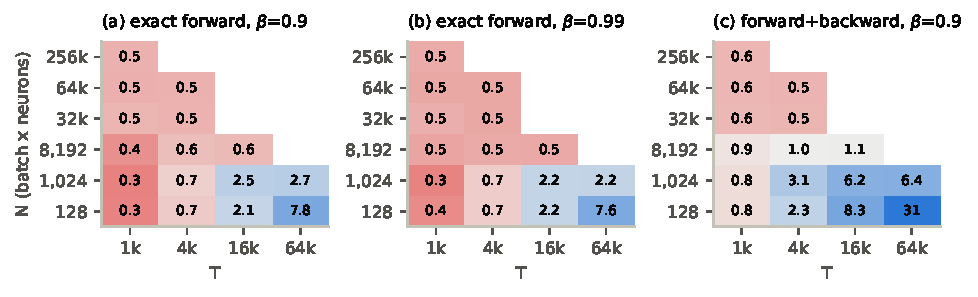
\includegraphics[width=\linewidth]{figs/gpu_speedup.pdf}
\caption{RTX~5090: speedup of the exact scan over the tuned fused serial kernel (both float32, both tuned per cell; ratios of median times; red means the scan is slower). $N$ is the number of independent recurrences (batch$\times$neurons). Inputs $\mathcal N(0.15,0.4^2)$, $u_r=0$, $\theta=1$; cells with $N\cdot T>2^{28}$ are omitted.}
\label{fig:gpu}
\end{figure}

\paragraph{Long sequences and three-level composition.}
On a second RTX~5090 node (same software stack), we extended the sequence length to $T=262{,}144$ and compared the two-level scan with the three-level variant, each again tuned per cell (Table~\ref{tab:long}). The two-level forward speedup grows with $T$, reaching $\LongFwdMaxNine\times$ ($\beta=0.9$) and $\LongFwdMaxNineNine\times$ ($\beta=0.99$) over the tuned serial kernel at $N=128$, $T=262{,}144$; forward+backward reaches $\LongFbMaxNine\times$. The three-level variant was exact in every cell (spike flips before repair: \LongMaxFlipNine), and its super-chunk maps, each composed from $G$ chunk maps covering up to 4096 steps, still had only a few pieces on average. It was nevertheless faster than the two-level scan in \LongVFourBestNine\ of the \LongCellsNine\ cells for $\beta=0.9$ and in \LongVFourBestNineNine\ of the \LongCellsNineNine\ cells for $\beta=0.99$. On this hardware and up to this length, the per-step carry is cheap enough that the extra $O(KK_2)$ composition work does not pay off, and the asymptotic depth advantage would only show at longer sequences.

\begin{table}[t]
\centering\small
\begin{tabular}{rrrrrrrr}
\toprule
$\beta$ & $N$ & $T$ & serial fwd (ms) & two-level & three-level & bwd $\times$ & fwd+bwd $\times$\\
\midrule
0.9 & 128 & 16{,}384 & 0.34 & 2.5$\times$ & 1.9$\times$ & 18$\times$ & 7.9$\times$\\
0.9 & 128 & 65{,}536 & 1.52 & 5.7$\times$ & 4.5$\times$ & 25$\times$ & 16$\times$\\
0.9 & 128 & 262{,}144 & 6.07 & 5.5$\times$ & 5.0$\times$ & 25$\times$ & 16$\times$\\
0.9 & 1{,}024 & 16{,}384 & 0.41 & 1.2$\times$ & 0.9$\times$ & 4.0$\times$ & 2.9$\times$\\
0.9 & 1{,}024 & 65{,}536 & 1.61 & 1.2$\times$ & 0.9$\times$ & 4.0$\times$ & 2.9$\times$\\
0.9 & 1{,}024 & 262{,}144 & 6.46 & 1.2$\times$ & 0.9$\times$ & 3.8$\times$ & 2.8$\times$\\
0.9 & 8{,}192 & 16{,}384 & 1.13 & 0.5$\times$ & 0.4$\times$ & 0.6$\times$ & 0.6$\times$\\
0.99 & 128 & 16{,}384 & 0.35 & 2.3$\times$ & 2.0$\times$ & 18$\times$ & 7.5$\times$\\
0.99 & 128 & 65{,}536 & 1.52 & 5.2$\times$ & 4.5$\times$ & 25$\times$ & 15$\times$\\
0.99 & 128 & 262{,}144 & 6.02 & 4.7$\times$ & 3.8$\times$ & 25$\times$ & 15$\times$\\
0.99 & 1{,}024 & 16{,}384 & 0.41 & 1.0$\times$ & 0.8$\times$ & 4.0$\times$ & 2.7$\times$\\
0.99 & 1{,}024 & 65{,}536 & 1.60 & 1.0$\times$ & 0.7$\times$ & 4.0$\times$ & 2.6$\times$\\
0.99 & 1{,}024 & 262{,}144 & 6.46 & 1.0$\times$ & 0.8$\times$ & 3.8$\times$ & 2.6$\times$\\
0.99 & 8{,}192 & 16{,}384 & 1.13 & 0.4$\times$ & 0.3$\times$ & 0.6$\times$ & 0.5$\times$\\
\bottomrule
\end{tabular}

\caption{Long sequences on the second RTX~5090 node. Columns 5--8 are speedups over the tuned serial kernel (forward: two-level and three-level exact scan; backward: affine scan; forward+backward: the better forward plus the scan backward). Each implementation is tuned per cell.}
\label{tab:long}
\end{table}

\paragraph{Forgetting in the adjoint.}
With a detached reset, $J_t=0$ at every spike, so the backward recurrence also forgets: a chunk that contains a spike has a composed slope of exactly $0$, and the scan's adjoint inside it is computed by the same instructions as the serial adjoint. On a 1024-step, 4096-neuron test with $\beta=0.95$, the scan's and the serial kernel's float32 adjoints have identical errors relative to a float64 reference ($1.3\times10^{-7}$), at every position within a chunk. Differences arise only from chunks without spikes.

\paragraph{SHD.}
We train a feed-forward 700--256--256--20 hard-reset LIF network ($\beta=0.95$) on the Spiking Heidelberg Digits~\citep{cramer2020shd} with 1\,ms bins ($T=1024$), batch 64, Adam (lr $10^{-3}$, cosine schedule) and 30 epochs, using the serial kernel, the scan (with repair), or SpikingJelly. On real batches with identical weights, the scan produces bit-identical spikes in both layers (\SpikesEqScanShort\ of 5 batches at $T=1024$, \SpikesEqScanLong\ at $T=8192$) and parameter gradients within $\GradRelScanShort$ ($T=1024$) and $\GradRelScanLong$ ($T=8192$) relative error of the serial kernel. SpikingJelly's gradients differ by up to $\GradRelSJShort$ and $\GradRelSJLong$, and at $T=8192$ a fraction up to $\SpikeMisSJLong$ of its spikes differ from the serial kernel's; serial vs.\ serial gives 0. Final test accuracies are $\AccSerial\%$ (serial, \NSeedsSerial\ seeds), $\AccScan\%$ (scan) and $\AccSJ\%$ (SpikingJelly), and the paired scan$-$serial difference is $\AccDiffScanSerial$ points (paired $t$-test $p=\AccDiffP$; Fig.~\ref{fig:shd}). Same-seed runs drift apart because $10^{-7}$ gradient differences are amplified over thousands of Adam steps; there is no difference in the dynamics. Repair is needed only for bit-identical \emph{membrane potentials}: without it, the first layer's spikes on 10 SHD batches still match the serial kernel's exactly (mismatch fraction \NoRepairMismatch). Repair nevertheless takes \RepairRoundsShort\ rounds at $T=1024$ and \RepairRoundsLong\ at $T=8192$, because with firing rates of \FireRateShort\% and \FireRateLong\% most chunks are silent and their affine parts differ from the serial loop by a few ulps. A long-sequence variant (0.12\,ms bins, $T=8192$, batch 16, 20 epochs, one seed) reaches $\AccLongSerial\%$ / $\AccLongScan\%$ / $\AccLongSJ\%$. Table~\ref{tab:shdtime} gives the per-iteration time of the whole network. Without repair, the scan is faster than the serial kernel for $T\ge4096$ and slower at $T=1024$; with repair, the extra replay rounds make it slower everywhere. SHD with $N=B\times256$ neurons per layer is a moderate workload. The scan helps when sequences are long and batches small, which is the latency-bound regime of Fig.~\ref{fig:gpu}.

\begin{table}[t]
\centering
\small
\begin{tabular}{rrrrrrrr}
\toprule
$T$ & batch & $N$/layer & serial & scan & scan, no repair & auto & SpikingJelly\\
\midrule
1024 & 8 & 2{,}048 & 1.2 & 2.6 & 1.4 & 1.2 & 1.9\\
1024 & 64 & 16{,}384 & 2.9 & 7.2 & 3.5 & 2.9 & 4.2\\
4096 & 16 & 4{,}096 & 4.9 & 12.0 & 3.7 & 3.4 & 10.7\\
8192 & 4 & 1{,}024 & 6.1 & 7.0 & 2.2 & 2.0 & 14.2\\
8192 & 16 & 4{,}096 & 9.2 & 37.1 & 7.3 & 6.3 & 21.1\\
\bottomrule
\end{tabular}

\caption{SHD network (two LIF layers plus linear maps), forward+backward time per iteration in ms (median of 10, RTX~5090). ``scan'' includes the bit-exactness repair, ``no repair'' omits it.}
\label{tab:shdtime}
\end{table}

\begin{figure}[t]
\centering
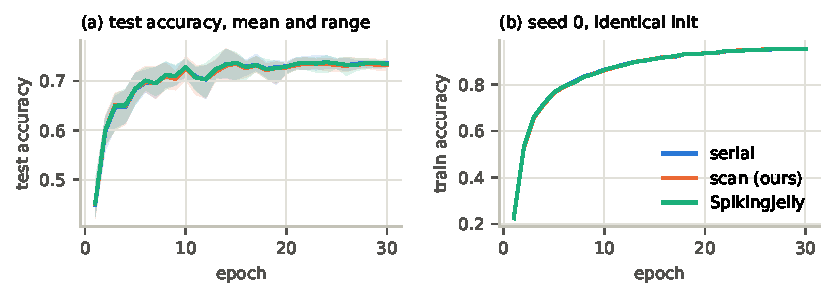
\includegraphics[width=0.92\linewidth]{figs/shd.pdf}
\caption{SHD training with the three kernels. (a) Test accuracy: mean and min--max over seeds. (b) Training accuracy of the seed-0 runs, which start from identical weights and data order.}
\label{fig:shd}
\end{figure}

\paragraph{SSC.}
To check that the equivalence does not depend on the dataset, we repeated the setup on the Spiking Speech Commands~\citep{cramer2020shd} (35 classes, 75{,}466 training samples), with the same network, $T=1024$, batch 64, 20 epochs and three seeds per kernel. On real batches with identical weights, the scan again produced \SscSpikesEqScan\ spikes bit-identical to the serial kernel, with gradient differences up to $\SscGradRelScan$ (SpikingJelly: $\SscGradRelSJ$). Final test accuracies are $\SscAccSerial\%$ (serial), $\SscAccScan\%$ (scan) and $\SscAccSJ\%$ (SpikingJelly), and the mean paired scan$-$serial difference is $\SscDiff$ points.

% ---------------------------------------------------------------------------
\section{Limitations and outlook}

\begin{itemize}[leftmargin=*]
\item \textbf{Regime.} Time-parallel evaluation pays only when serial evaluation leaves the GPU idle. With large batch$\times$width, a well-tuned serial kernel is faster. In our measurements, the exact forward wins for $N\le1$k at $T\ge16$k, forward+backward breaks even near $N\approx8$k, and for $N\ge32$k the scan runs at about half the serial speed.
\item \textbf{Within-layer recurrence.} The method needs the input currents of a layer for all $t$ in advance; recurrent synaptic connections within a layer break this, as they do for every scan-based method. Current-based synapses are not a problem: the synaptic current is a linear filter of the inputs and can be scanned first.
\item \textbf{Silent integrators.} With the envelope bound, map sizes are small in every regime we measured except $\beta\to1$ with near-zero drift, where they grow like $\sqrt L$ and overflow becomes more frequent. The output stays exact, but the speed degrades towards serial. A three-level variant reduces the depth further and is exact, but on our hardware it did not beat the two-level scan up to $T=262{,}144$ (Table~\ref{tab:long}).
\item \textbf{Other neurons.} For adaptive-threshold (ALIF) neurons the reset acts on one coordinate of a two-dimensional state, forgetting is only partial, and the pieces of a segment map become polygons in the $(u_0,w_0)$ plane. A sampling estimate (App.~\ref{app:extra}, Table~\ref{tab:alif}) suggests that their number grows only moderately with $L$ (about 15--22 regions at $L=64$ on a fixed window, against 7 for LIF), so map-space scans may extend to them. A compact representation of polygonal maps and a structure theorem are the main open problems.
\item \textbf{Floating point and deployment.} Bit-exactness is with respect to a serial program in the same arithmetic. Deploying to fixed-point neuromorphic hardware still requires simulation in that hardware's arithmetic.
\end{itemize}

\paragraph{Conclusion.}
The hard reset does not prevent associative scans; it only requires scanning maps rather than states. The resulting maps are small and well structured --- linear in the worst case, a handful of pieces once pruned to the reachable states, and simpler than their soft-reset counterparts --- and they yield an exact, non-iterative parallel forward pass for LIF neurons whose depth does not depend on the number of spikes.

\bibliographystyle{plainnat}
\bibliography{refs}

% ---------------------------------------------------------------------------
\appendix
\section{Proof of Theorem~\ref{thm:soft}}
\label{app:soft}

Fix $u_0<u_0'$, write primes for the trajectory from $u_0'$, and let $d_t=N'_t-N_t$, $\Phi_t=(u'_t+\theta N'_t)-(u_t+\theta N_t)$.

\begin{lemma}
For all $t\ge0$: $d_t\ge0$ and $\Phi_t>0$. Consequently $N_t(\cdot)$ is non-decreasing, and $N_t(u_0)=N_t(u_0')$ implies $u_t(u_0)<u_t(u_0')$.
\end{lemma}
\begin{proof}
At $t=0$, $d_0=0$ and $\Phi_0=u'_0-u_0>0$. From $u_t=v_t-\theta s_t$ and $N_t=N_{t-1}+s_t$ we get $u_t+\theta N_t=\beta u_{t-1}+I_t+\theta N_{t-1}$, hence
$\Phi_t=\beta(u'_{t-1}-u_{t-1})+\theta d_{t-1}=\beta\Phi_{t-1}+(1-\beta)\theta d_{t-1}$,
which is positive because $\beta>0$, $\Phi_{t-1}>0$, $1-\beta\ge0$, $\theta>0$ and $d_{t-1}\ge0$.
For $d_t$: if $d_{t-1}\ge1$ then $N_t\le N_{t-1}+1\le N'_{t-1}\le N'_t$; if $d_{t-1}=0$ then $u'_{t-1}-u_{t-1}=\Phi_{t-1}>0$, so $v'_t>v_t$ and $s'_t\ge s_t$.
\end{proof}

Between breakpoints all $s_j$ are constant and $u_L$ is affine with slope $\beta^L$, so breakpoints occur only where some $s_t$ changes. Call a point a \emph{new breakpoint of step $t$} if $s_t$ changes there while $s_1,\ldots,s_{t-1}$ do not; there $u_{t-1}$ is continuous and equals $c_t=(\theta-I_t)/\beta$. By the lemma, the level sets of $N_{t-1}$ are intervals on which $u_{t-1}$ is strictly increasing, so each contains at most one solution of $u_{t-1}=c_t$. Since $N_{t-1}\in\{0,\ldots,t-1\}$, step $t$ creates at most $t$ new breakpoints, and the total is at most $\sum_{t=1}^Lt$. \qed

\section{Proof of Theorem~\ref{thm:softtight}}
\label{app:softtight}

Write $x=u_0$ and $g_t(x)=\lfloor (x+tI)/\theta\rfloor$.

\emph{Step 1 ($\beta=1$).} By induction on $t$, $N_t(x)=\min(t,\max(0,g_t(x)))$. With $\beta=1$, $v_t=x+tI-\theta N_{t-1}$, so $s_t=1$ iff $N_{t-1}+1\le (x+tI)/\theta$, i.e.\ iff $g_t\ge N_{t-1}+1$. Since $0<I<\theta$, $g_t\in\{g_{t-1},g_{t-1}+1\}$. If $N_{t-1}=0\ge g_{t-1}$, the neuron fires iff $g_t=1$. If $N_{t-1}=t-1\le g_{t-1}$, it fires iff $g_t\ge t$. Otherwise $N_{t-1}=g_{t-1}$, and it fires iff $g_t=g_{t-1}+1$. In each case $N_t=\min(t,\max(0,g_t))$.

Hence each $N_t(\cdot)$ is a non-decreasing step function whose jumps are exactly at $x_{t,k}=k\theta-tI$, $1\le k\le t$. By the assumption on $I/\theta$ these $L(L+1)/2$ points are distinct, since $x_{t,k}=x_{t',k'}$ with $t\ne t'$ would give $I/\theta=(k-k')/(t-t')$. They split $\mathbb R$ into $M=1+L(L+1)/2$ open intervals. On each interval the spike pattern $P=(s_1,\ldots,s_L)$ is constant, and the patterns of different intervals are distinct, because $(N_1,\ldots,N_L)$ increases componentwise across every switch point. Moreover $v_t(x)=\theta$ only at the switch point $x_{t,N_{t-1}+1}$, so inside each interval every threshold comparison is strict.

\emph{Step 2 (perturbation).} For a pattern $P$, let $v^{P,\beta}_t(x)=\beta^tx+b_t(\beta)-\theta\sum_{j<t}s_j\beta^{t-j}$ be the pre-reset potential when the spikes of $P$ are imposed. The set of $x$ whose actual pattern is $P$ is $R_P(\beta)=\{x:\ [v^{P,\beta}_t(x)\ge\theta]=s_t\ \forall t\}$. It is an interval, since each constraint is a half-line in $x$. Pick $x_P$ inside the interval of $P$ at $\beta=1$. All constraints hold strictly at $(x_P,1)$ and are continuous in $\beta$, so for $\beta\in(1-\delta,1]$ they hold strictly in a neighbourhood of $x_P$. Thus all $M$ patterns are realized on intervals of positive length.

\emph{Step 3 (distinct pieces).} On $R_P(\beta)$, $u_L(x)=\beta^Lx+b_L(\beta)-\theta\rho_P(\beta)$ with $\rho_P(\beta)=\sum_js_j\beta^{L-j}$. For $P\ne P'$, $\rho_P-\rho_{P'}$ is a non-zero polynomial with coefficients in $\{-1,0,1\}$, so it vanishes for finitely many $\beta$ only. Away from these values, the $M$ disjoint intervals carry affine functions with equal slopes and pairwise distinct intercepts. Hence the map has at least $M$ pieces, and by Theorem~\ref{thm:soft} exactly $M$. \qed

\section{Additional results}
\label{app:extra}

Table~\ref{tab:e1} lists piece counts of exact segment maps for hard and soft reset, Table~\ref{tab:stress} the near-threshold floating-point stress test, and Table~\ref{tab:alif} the region counts for adaptive-threshold neurons.

\begin{table}[!htbp]
\centering\small
\begin{tabular}{rrrrrrr}
\toprule
$\beta$ & $\mu$ & $L$ & hard mean (max) & bound & soft mean (max) & bound\\
\midrule
0.5 & 0.05 & 8 & 2.1 (3) & 9 & 9.3 (11) & 37\\
0.5 & 0.05 & 32 & 2.2 (4) & 33 & 36.7 (47) & 529\\
0.5 & 0.3 & 8 & 2.7 (5) & 9 & 12.5 (20) & 37\\
0.5 & 0.3 & 32 & 2.8 (5) & 33 & 48.5 (58) & 529\\
0.9 & 0.05 & 8 & 3.7 (6) & 9 & 16.5 (29) & 37\\
0.9 & 0.05 & 32 & 4.8 (11) & 33 & 85.2 (198) & 529\\
0.9 & 0.3 & 8 & 5.8 (7) & 9 & 25.8 (32) & 37\\
0.9 & 0.3 & 32 & 9.8 (18) & 33 & 196.6 (286) & 529\\
0.99 & 0.05 & 8 & 4.7 (9) & 9 & 22.4 (37) & 37\\
0.99 & 0.05 & 32 & 8.0 (11) & 33 & 165.5 (314) & 529\\
0.99 & 0.3 & 8 & 6.0 (8) & 9 & 28.4 (37) & 37\\
0.99 & 0.3 & 32 & 11.9 (19) & 33 & 377.1 (435) & 529\\
\bottomrule
\end{tabular}

\caption{Pieces of exact segment maps on random inputs $I_t\sim\mathcal N(\mu,0.3^2)$ (quantized to $10^{-3}$, 20 draws per row, rational arithmetic).}
\label{tab:e1}
\end{table}

\begin{table}[!htbp]
\centering\small
\begin{tabular}{rrrrr}
\toprule
$\beta$ & $\varepsilon$ & flips scan32 vs serial32 & flips serial32 vs serial64 & repair rounds\\
\midrule
0.9 & $10^{-5}$ & 0 & 0.23\% & 0\\
0.9 & $10^{-6}$ & 0 & 2.12\% & 0\\
0.9 & $10^{-7}$ & 0 & 14.56\% & 0\\
0.99 & $10^{-5}$ & 0 & 0.26\% & 0\\
0.99 & $10^{-6}$ & 0 & 2.49\% & 0\\
0.99 & $10^{-7}$ & 0 & 15.89\% & 0\\
\bottomrule
\end{tabular}

\caption{Near-threshold stress test (PyTorch prototype on CPU, $T=4096$, 512 neurons; 30\% of the steps are constructed so that the float64 pre-reset potential lies within $\pm\varepsilon$ of $\theta$). Columns 3--4 give the fraction of spike entries that differ. Float32 vs.\ float64 disagreement is the intrinsic rounding noise of the serial recurrence; the scan adds none.}
\label{tab:stress}
\end{table}

\begin{table}[!htbp]
\centering\small
\begin{tabular}{lrrrrr}
\toprule
model & $L=4$ & $L=8$ & $L=16$ & $L=32$ & $L=64$\\
\midrule
LIF & 2.6 (4) & 5.0 (6) & 5.0 (7) & 5.4 (8) & 7.0 (9)\\
ALIF $q=$0.5 & 3.6 (5) & 4.4 (6) & 7.0 (10) & 12.6 (18) & 15.4 (28)\\
ALIF $q=$1.0 & 2.4 (4) & 4.8 (8) & 11.8 (15) & 13.4 (21) & 22.0 (33)\\
\bottomrule
\end{tabular}

\caption{Number of distinct spike patterns (= affine pieces) of the $L$-step map on the window $u_0\in[-4,1]$, $w_0\in[0,2]$, estimated on a $700\times700$ grid, mean and max over 5 random inputs $\mathcal N(0.15,0.4^2)$. $\beta=0.9$, $\theta_0=1$, $u_r=0$; ALIF threshold $\theta_0+w_{t-1}$ with $w_t=0.95\,w_{t-1}+q\,s_t$. Sampling gives a lower bound.}
\label{tab:alif}
\end{table}

\section{Implementation details}
\label{app:impl}

\paragraph{Kernels.} All kernels share one step function, so the serial kernel and the replay execute identical instructions (including FMA contraction). Envelope: one kernel composes the $\min(c,au+b)$ maps of each chunk, and a second carries $l$ across chunks; a relative margin of $10^{-5}$ is subtracted from $l$ to absorb rounding. Build: grid (chunks, neuron blocks); each program keeps $A,B$, the breakpoints (in descending order) and constants of its maps in registers as a $[\text{BN},K]$ tile. Carry: one program per neuron block evaluates $M$ maps by counting breakpoints above the state and gathering the constant. Replay and the serial baseline: time-tiled ($D$ steps per tile, next tile prefetched). Backward: chunk-composed affine maps, a carry over chunks, and a tiled reverse replay.

\paragraph{Tuning grids.} Configurations are written as (block size BN, tile depth $D$, warps).
\begin{itemize}[leftmargin=*]
\item Serial forward and backward: plain, or tiled with (32,4,1), (64,4,2), (32,8,1) or (128,4,4).
\item Scan forward: $C\in\{32,64,128,256\}$ and $K\in\{8,16,32\}$; build with (32,--,1) or (128,--,4); replay with (32,8,1) or (64,4,2).
\item Scan backward: the same $C$, with the serial tilings.
\end{itemize}
All configurations of every implementation are timed in the same process. Reported times are medians of 7 runs after warm-up, and every reported scan configuration was checked for spike flips against the serial kernel.

\paragraph{Reproducibility.} The repository contains the exact reference, all experiment scripts, raw JSON results and a queue script that regenerates every GPU number.

\end{document}
